%\documentclass[12pt,preprint]{aastex}
\documentclass[iop,apj]{emulateapj}
\usepackage{multirow}
\usepackage{longtable}
\usepackage{ulem}
%\usepackage[monochrome]{color}
\usepackage{color}
\usepackage{lipsum}
\usepackage{amsmath}
%\usepackage{hyperref}

\newcommand{\eqqref}[1]{Equation (\ref{#1})}
\newcommand{\tabref}[1]{Table~\ref{#1}}
\newcommand{\figref}[1]{Figure~\ref{#1}}
\newcommand{\secref}[1]{Section~\ref{#1}}
\newcommand{\appref}[1]{Appendix~\ref{#1}}

\newcommand{\SNeIa}{SNe~Ia}
\newcommand{\SNIa}{SN~Ia}
\newcommand{\C}[1]{\ensuremath{{}^{#1}{\rm C}}}
\newcommand{\Ox}[1]{\ensuremath{{}^{#1}{\rm O}}}
\newcommand{\Ne}[1]{\ensuremath{{}^{#1}{\rm Ne}}}
\newcommand{\Na}[1]{\ensuremath{{}^{#1}{\rm Na}}}
\newcommand{\Mg}[1]{\ensuremath{{}^{#1}{\rm Mg}}}
\newcommand{\Ni}[1]{\ensuremath{{}^{#1}{\rm Ni}}}
\newcommand{\Co}[1]{\ensuremath{{}^{#1}{\rm Co}}}
\newcommand{\Si}[1]{\ensuremath{{}^{#1}{\rm Si}}}
\newcommand{\Fe}[1]{\ensuremath{{}^{#1}{\rm Fe}}}
\newcommand{\code}[1]{\textsc{#1}}
\newcommand{\FLASH}{\code{FLASH}}
\newcommand{\CASTRO}{\code{CASTRO}}
\newcommand{\MESA}{\code{MESA}}
\newcommand{\PARAMESH}{\code{PARAMESH}}
\newcommand{\pv}{\ensuremath{\phi}}
\newcommand{\bvec}[1]{\ensuremath{\boldsymbol{#1}}} %boldface vector style
\newcommand{\grad}{\bvec{\nabla}} %gradient
\newcommand{\curl}{\bvec{\nabla \times}} %curl
\newcommand{\Atwood}{\ensuremath{\mathrm{At}}}
\newcommand{\adndt}{At.~Data~Nucl.~Data~Tables}
\newcommand{\At}{{\rm At}}
\newcommand{\ee}[1]{\ensuremath{\times 10^{#1}}}
\newcommand{\cdens}{\rho_{c}}

% basic unit typesetteing
\newcommand{\unitspace}{\ensuremath{\,}}
\newcommand{\usp}{\unitspace}
\newcommand{\numberspace}{\ensuremath{\;}}
\newcommand{\nsp}{\numberspace}
\newcommand{\unitstyle}[1]{\ensuremath{\mathrm{#1}}}
\newcommand{\power}[2]{\ensuremath{{#1}^{#2}}}


% prefixes
\newcommand{\nano}{\unitstyle{n}}
\newcommand{\milli}{\unitstyle{m}}
\newcommand{\centi}{\unitstyle{c}}
\newcommand{\kilo}{\unitstyle{k}}
\newcommand{\Mega}{\unitstyle{M}}
\newcommand{\Giga}{\unitstyle{G}}

% base units, mks
\newcommand{\meter}{\unitstyle{m}}
\newcommand{\kilogram}{\kilo\gram}
\newcommand{\second}{\unitstyle{s}}

\newcommand{\Kelvin}{\unitstyle{K}}
\newcommand{\K}{\Kelvin}  %degrees Kelvin


% base units, cgs
\newcommand{\cm}{\centi\meter}
\newcommand{\gram}{\unitstyle{g}}


% derived units
\newcommand{\grampercc}{\gram\usp\power{\cm}{-3}} %mass density
\newcommand{\grampersquarecm}{\gram\usp\power{\cm}{-2}} %column depth
\newcommand{\GramPerCc}{\grampercc}
\newcommand{\GramPerSc}{\grampersquarecm}
\newcommand{\columnunit}{\grampersquarecm}
\newcommand{\dyne}{\unitstyle{dyn}} %dyne
\newcommand{\erg}{\unitstyle{ergs}} %ergs
\newcommand{\ergs}{\erg}
\newcommand{\gauss}{\unitstyle{G}} %gauss
\newcommand{\ergspersecond}{\erg\unitspace\power{\second}{-1}}
\newcommand{\ergspergram}{\erg\unitspace\power{\gram}{-1}}
\newcommand{\cgsflux}{\erg\unitspace\power{\cm}{-2}\usp\power{\second}{-1}}
\newcommand{\kms}{\kilo\meter\unitspace\power{\second}{-1}}

% Nuclear and atomic units
\newcommand{\amu}{\unitstyle{u}} %atomic mass unit
\newcommand{\angstrom}{\mbox{\AA}} %Angstrom
\newcommand{\fermi}{\unitstyle{fm}} %fermi
\newcommand{\eV}{\unitstyle{eV}}        %eV
\newcommand{\keV}{\kilo\eV} %Kev
\newcommand{\MeV}{\Mega\eV} %MeV

% solar and astronomical units
\newcommand{\Msun}{\ensuremath{M_\odot}}
\newcommand{\Myr}{\Mega\yr}
\newcommand{\Gyr}{\Giga\yr}
\newcommand{\parsec}{\unitstyle{pc}}
\newcommand{\kpc}{\kilo\parsec} %kiloparsec
\newcommand{\mJy}{\unitstyle{\mu Jy}} %micro Jansky

% misc. units
\newcommand{\minute}{\unitstyle{min}} %minute
\newcommand{\hour}{\unitstyle{hr}} %hour
\newcommand{\yr}{\unitstyle{yr}}        %year
\newcommand{\km}{\kilo\meter}   %kilometers
\newcommand{\Hz}{\unitstyle{Hz}}        %Hertz
\newcommand{\ksec}{\kilo\second} %kilosecond

\newcommand{\tDDT}{\ensuremath{t_{\rm DDT}}}
\newcommand{\rhoDDT}{\ensuremath{\rho_{\rm DDT}}}
\newcommand{\COreac}{\ensuremath{\C{12}\left(\alpha,\gamma\right)\Ox{16}}}

\bibliographystyle{apj}

\shorttitle{Short Paper Title}

\begin{document}

\title{Paper Title}

\author{
Some Awesome People\altaffilmark{1,2,3,4}
}

\altaffiltext{1}{
  Department of Physics and Astronomy,
  Stony Brook University, Stony Brook, NY, 11794-3800, USA; \\
  \href{mailto:somebody@someplace}{somebody@someplace}
}
\altaffiltext{2}{
  Department of Physics and Astronomy,
  The University of Alabama, Tuscaloosa, AL, 35487-0324, USA
}
\altaffiltext{3}{
  Department of Physics and Astronomy,
  Stony Brook University, Stony Brook, NY, 11794-3800, USA
}
\altaffiltext{4}{
  Institute for Advanced Computational Sciences,
  Stony Brook University, Stony Brook, NY, 11794-5250, USA
}

\begin{abstract}
Awesome Abstract
\end{abstract}

\keywords{hydrodynamics --- nuclear reactions, nucleosynthesis, abundances
--- supernovae: general --- white dwarfs}

%%%%%%%%%%%%%%%%%%%%%%%%%%%%%%%%%%%%%%%%%%%%%%%%%%%%%%%%%%%%%%%%%%
\section{Introduction}
\label{sec:intro}

Introduction with a pretty plot in \figref{fig:progenitor_abundances}.

\begin{figure}[t]
	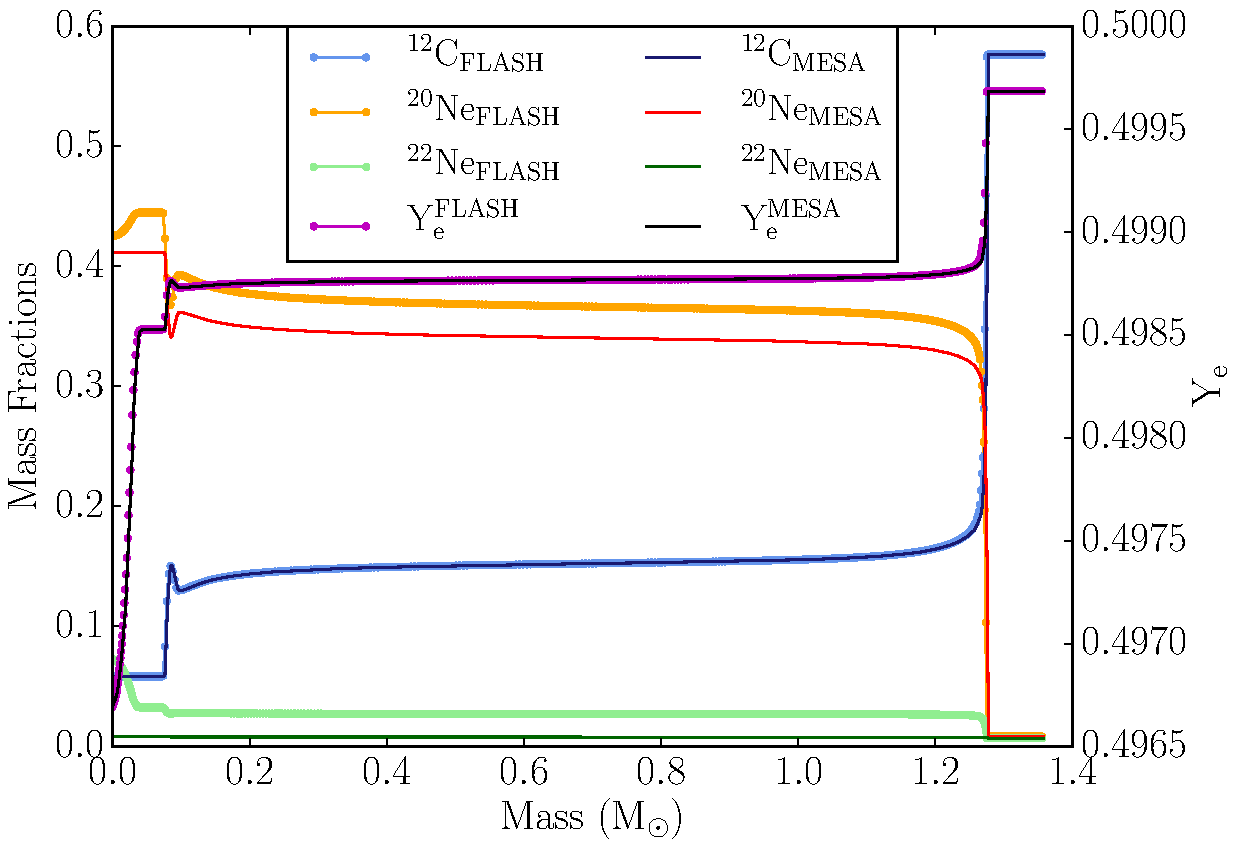
\includegraphics[width=\linewidth]{figures/samples/cf_wdb_mesa_comp_vs_mass.pdf}
	\caption{\label{fig:progenitor_abundances} Abundance profile
          of \MESA\ progenitor (\MESA) and its reconstruction on a
          uniform grid at $4$~km spatial resolution with the hydrostatic equilibrium condition of
          \eqqref{eq:hse_pressure} enforced (\FLASH). The reduced set
          of nuclides are shown, where $\mathrm{X_{\Ox{16}} = 1 -
            X_{\C{12}} - X_{\Ne{20}} - X_{\Ne{22}}}$ for the
          abundances labeled \FLASH. Solid lines and circles denote
          the abundances used in \FLASH\ whereas plain solid lines
          denote the abundances used in \MESA.}
\end{figure}

\section{Methodology}

Methodology goes here.

A handy example of a vertical multi-plot figure is \figref{fig:znd_abundances}.

\begin{figure}[t]
	\begin{minipage}{0.5\textwidth}
		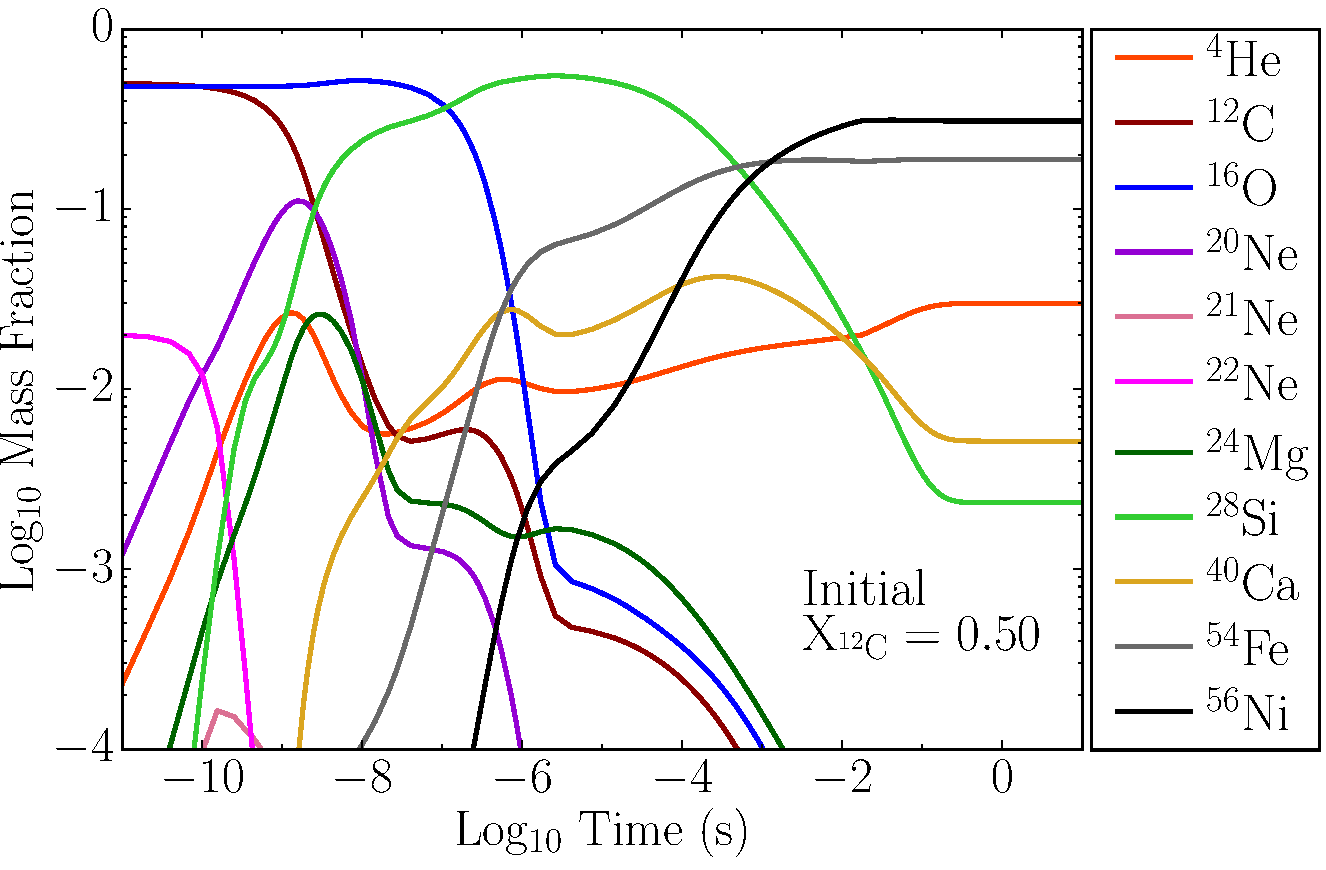
\includegraphics[width=0.86\textwidth]{figures/samples/XvsT_wn_0_XC-50.pdf}
		%\caption{\label{fig:znd_abundances_xc12_0.5} Initial composition: $X_{^{16}O} = 0.48$, $X_{^{22}Ne} = 0.02$, $X_{^{12}C} = 0.50$, $X_{^{20}Ne} = 0.00$}
	\end{minipage}	
	\hfill
	\begin{minipage}{0.5\textwidth}
		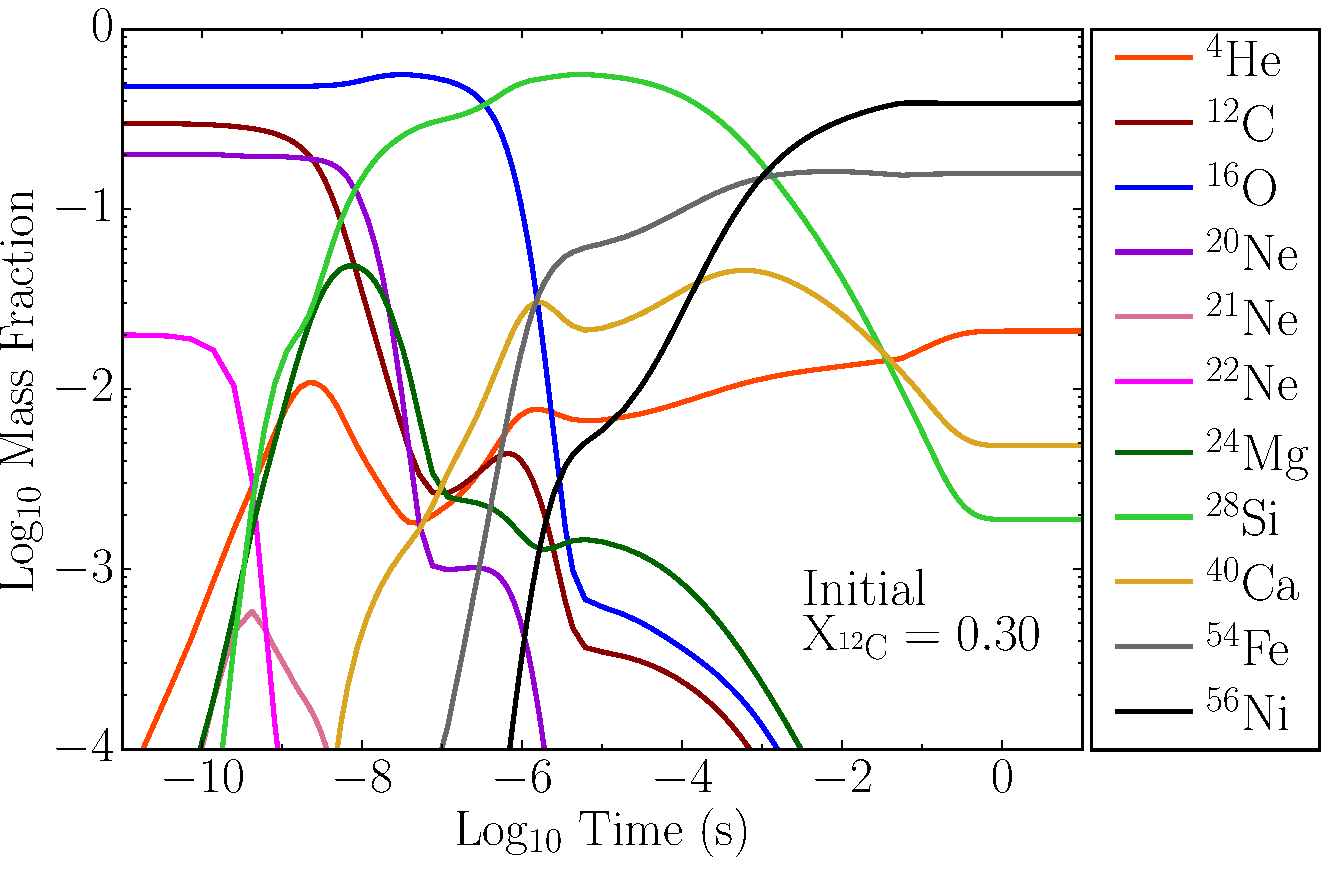
\includegraphics[width=0.86\textwidth]{figures/samples/XvsT_wn_20_XC-30.pdf}
		%\caption{\label{fig:znd_abundances_xc12_0.3} Initial composition: $X_{^{16}O} = 0.48$, $X_{^{22}Ne} = 0.02$, $X_{^{12}C} = 0.30$, $X_{^{20}Ne} = 0.20$}
	\end{minipage}
	\hfill
	\begin{minipage}{0.5\textwidth}
		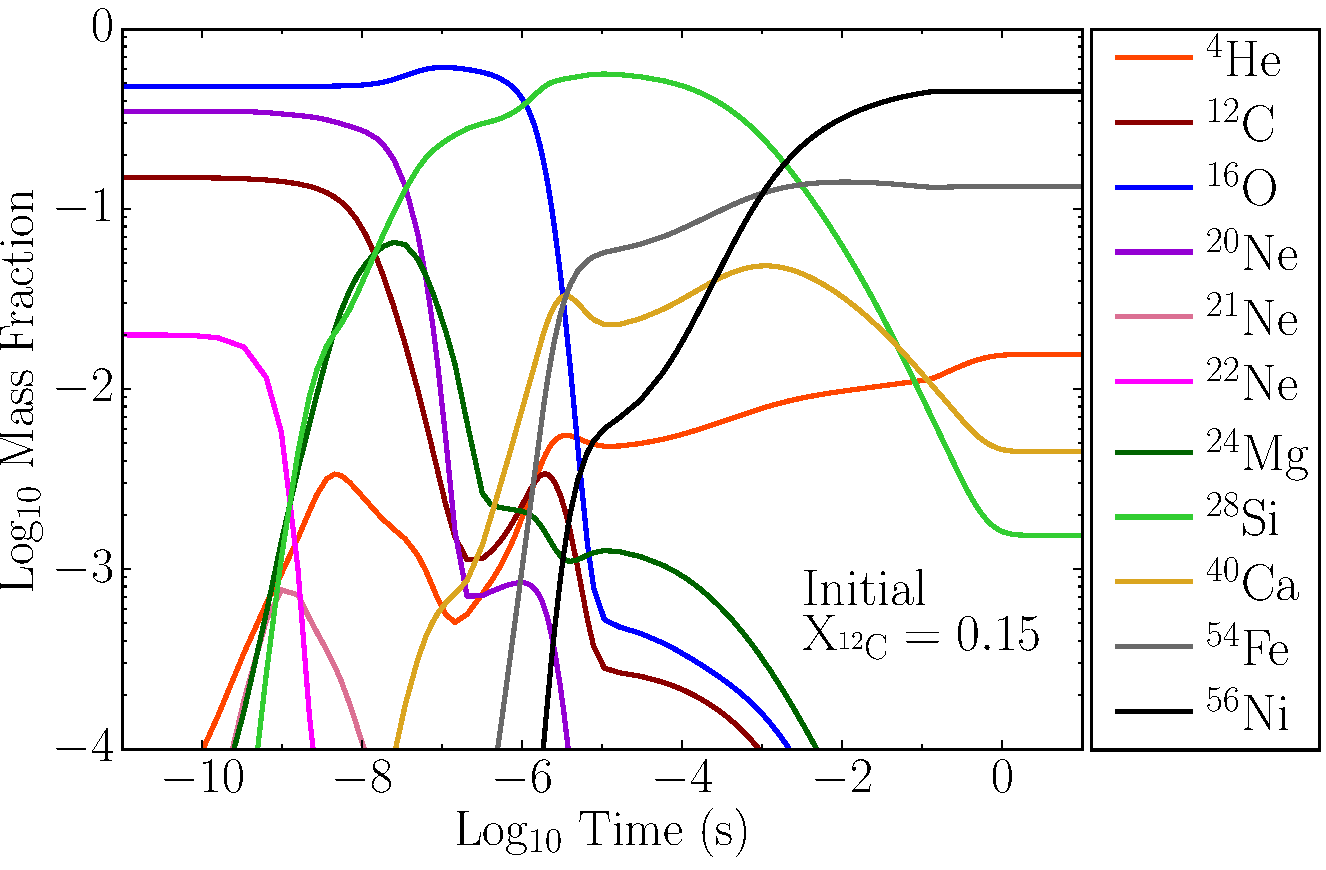
\includegraphics[width=0.86\textwidth]{figures/samples/XvsT_wn_35_XC-15.pdf}
		%\caption{\label{fig:znd_abundances_xc12_0.15} Initial composition: $X_{^{16}O} = 0.48$, $X_{^{22}Ne} = 0.02$, $X_{^{12}C} = 0.15$, $X_{^{20}Ne} = 0.35$}
	\end{minipage}
	\hfill
	\begin{minipage}{0.5\textwidth}
		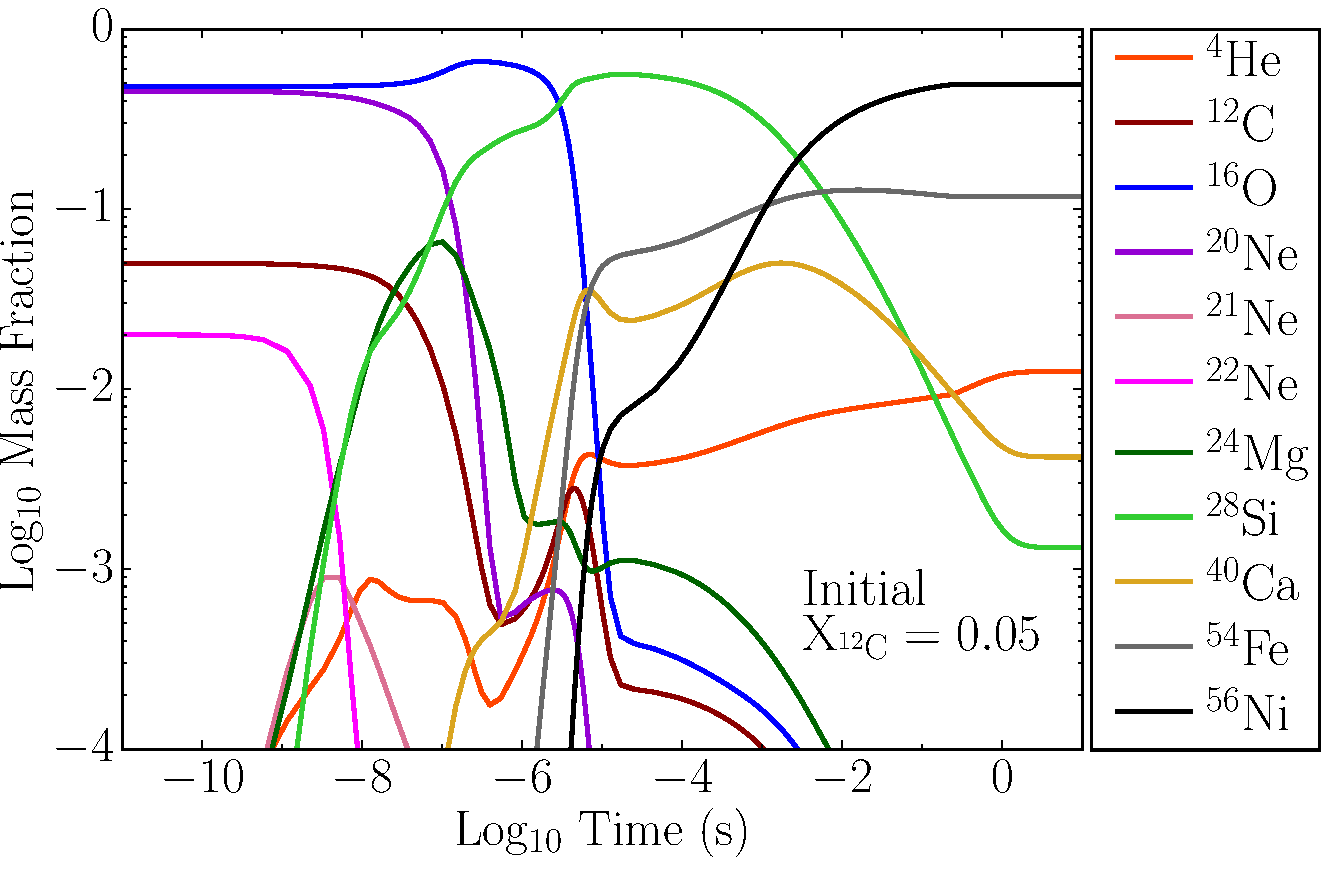
\includegraphics[width=0.86\textwidth]{figures/samples/XvsT_wn_45_XC-05.pdf}
		%\caption{\label{fig:znd_abundances_xc12_0.05} Initial composition: $X_{^{16}O} = 0.48$, $X_{^{22}Ne} = 0.02$, $X_{^{12}C} = 0.05$, $X_{^{20}Ne} = 0.45$}
	\end{minipage}
        \caption{\label{fig:znd_abundances} Mass Fraction Evolution for ZND Detonations with varying initial \C{12} and \Ne{20} mass fractions, calculated for an initial density of $10^7~\grampercc$.}
\end{figure}

Here's a text citation \citet{timmes92,Chametal08}, and here's a parenthetical citation ~\citep{timmes.swesty:accuracy,castro1}.

Here's an ordinary equation in \eqref{eq:hse_pressure}.

\begin{equation}\label{eq:hse_pressure}
  P_{EOS}(\rho_i,T_i,X_i) = \frac{g \Delta r}{2} (\rho_i +
  \rho_{i-1})\ .
\end{equation}

Here's a multi-line equation.

\begin{subequations}
\begin{align}
X_{\C{12}}^{FLASH} &= X_{\C{12}}^{MESA} \\
X_{\Ne{22}}^{FLASH} &= 22 \cdot \left(\dfrac{1}{2}-Y_e^{MESA}\right) \\
R &= X_{\Ne{20}}^{MESA}/X_{\Ox{16}}^{MESA} \\
X_{\Ox{16}}^{FLASH} &= \frac{1 - X_{\C{12}}^{FLASH} - X_{\Ne{22}}^{FLASH}}{R + 1} \\
X_{\Ne{20}}^{FLASH} &= R \cdot X_{\Ox{16}}^{FLASH}.
\end{align}
\end{subequations}

\section{Simulations and Results}

Simulations and results go here.

Example of multi-figure plot that spans the columns is given by \figref{fig:cone_delayed_core}.

\begin{figure*}[!ht]
  \begin{minipage}{0.24\textwidth}
    \includegraphics[width=\linewidth]{"figures/samples/cone_400k_m16_a12_0000"}
  \end{minipage} \hfill
  \begin{minipage}{0.24\textwidth}
    \includegraphics[width=\linewidth]{"figures/samples/cone_400k_m16_a12_0190"}
  \end{minipage} \hfill 
  \begin{minipage}{0.24\textwidth}
    \includegraphics[width=\linewidth]{"figures/samples/cone_400k_m16_a12_0200"}
  \end{minipage} \hfill 
  \begin{minipage}{0.24\textwidth}
    \includegraphics[width=\linewidth]{"figures/samples/cone_400k_m16_a12_0210"}
  \end{minipage} \caption{\label{fig:cone_delayed_core} Progress of the burning front into the stellar core for one hybrid C-O-Ne realization, delayed relative to complete burning throughout the rest of the star. For reference, the initially burned geometry is shown at left. Material is shaded based on the reaction progress variables so that \textbf{White} denotes unburned fuel (\C{12}, \Ox{16} \& \Ne{20}) and \textbf{Red} denotes ash from \C{12} and \Ne{20}-burning. \textbf{Green} then denotes material in quasi-nuclear statistical equilibrium (primarily intermediate-mass silicon-group elements), and \textbf{Black} denotes material in nuclear statistical equilibrium (IGEs and $\alpha$-particles). From left to right, the burning is shown at 0.0~\second, 1.9~\second, 2.0~\second, and 2.1~\second. The DDT time for this realization is $\approx \mathrm{1.4}~\second$.}
\end{figure*}

Example of a table with data, units, etc is at \tabref{YieldSummaryTable}.

\begin{table}[htbp]
  \caption{Average Yields and Kinetic Energy}
  \begin{center}
    \begin{tabular}{llll}
      \vspace{-0.75cm} \\ \hline \hline
      Progenitor & \Ni{56} & IGE & Kinetic Energy \\
      Type & (\Msun) & (\Msun) & $\left(\times 10^{51} ~\erg\right)$ \\ \hline
      C-O & $0.97 \pm 0.06$ & $1.12 \pm 0.07$ & $1.39 \pm 0.05$ \\
      C-O-Ne & $0.86 \pm 0.10$ & $0.98 \pm 0.11$ & $1.06 \pm 0.10$ \\ \hline
    \end{tabular}
  \end{center}
  \label{YieldSummaryTable}
\end{table}



%%%%%%%%%%%%%%%%%%%%%%%%%%%%%%%%%%%%%%%%%%%%%%%%%%%%%%%%%%%%%%%%%%
\section{Conclusions}
\label{sec:conclusions}

Conclusive conclusions go here.

\section{Appendix}

If there's material for an appendix, it can go here.

%%%%%%%%%%%%%%%%%%%%%%%%%%%%%%%%%%%%%%%%%%%%%%%%%%%%%%%%%%%%%%%%%%
\acknowledgements

We'd like to acknowledge helpful discussions with Cab Ernet.

%%%%%%%%%%%%%%%%%%%%%%%%%%%%%%%%%%%%%%%%%%%%%%%%%%%%%%%%%%%%%%%%%%
% SOFTWARE
%% \software{
%%   FLASH \citep{Fryxetal00},
%%   CASTRO \citep{castro1},
%%   MESA \citep{mesa1},
%%   Matplotlib \citep{http://dx.doi.org/10.5281/zenodo.44579}
%% }

%%%%%%%%%%%%%%%%%%%%%%%%%%%%%%%%%%%%%%%%%%%%%%%%%%%%%%%%%%%%%%%%%%
\bibliography{master}

\end{document}

